% Options for packages loaded elsewhere
\PassOptionsToPackage{unicode}{hyperref}
\PassOptionsToPackage{hyphens}{url}
%
\documentclass[
  ignorenonframetext,
  aspectratio=169]{beamer}
\title{Experimental designs}
\author{Deependra Dhakal}
\date{}
\institute{Assistant Professor \and Agriculture and Forestry
University \and \url{https://rookie.rbind.io}}

\usepackage{pgfpages}
\setbeamertemplate{caption}[numbered]
\setbeamertemplate{caption label separator}{: }
\setbeamercolor{caption name}{fg=normal text.fg}
\beamertemplatenavigationsymbolsempty
% Prevent slide breaks in the middle of a paragraph
\widowpenalties 1 10000
\raggedbottom
\setbeamertemplate{part page}{
  \centering
  \begin{beamercolorbox}[sep=16pt,center]{part title}
    \usebeamerfont{part title}\insertpart\par
  \end{beamercolorbox}
}
\setbeamertemplate{section page}{
  \centering
  \begin{beamercolorbox}[sep=12pt,center]{part title}
    \usebeamerfont{section title}\insertsection\par
  \end{beamercolorbox}
}
\setbeamertemplate{subsection page}{
  \centering
  \begin{beamercolorbox}[sep=8pt,center]{part title}
    \usebeamerfont{subsection title}\insertsubsection\par
  \end{beamercolorbox}
}
\AtBeginPart{
  \frame{\partpage}
}
\AtBeginSection{
  \ifbibliography
  \else
    \frame{\sectionpage}
  \fi
}
\AtBeginSubsection{
  \frame{\subsectionpage}
}
\usepackage{amsmath,amssymb}
\usepackage{lmodern}
\usepackage{iftex}
\ifPDFTeX
  \usepackage[T1]{fontenc}
  \usepackage[utf8]{inputenc}
  \usepackage{textcomp} % provide euro and other symbols
\else % if luatex or xetex
  \usepackage{unicode-math}
  \defaultfontfeatures{Scale=MatchLowercase}
  \defaultfontfeatures[\rmfamily]{Ligatures=TeX,Scale=1}
\fi
\usetheme[]{Frankfurt}
\usecolortheme{beaver}
% Use upquote if available, for straight quotes in verbatim environments
\IfFileExists{upquote.sty}{\usepackage{upquote}}{}
\IfFileExists{microtype.sty}{% use microtype if available
  \usepackage[]{microtype}
  \UseMicrotypeSet[protrusion]{basicmath} % disable protrusion for tt fonts
}{}
\makeatletter
\@ifundefined{KOMAClassName}{% if non-KOMA class
  \IfFileExists{parskip.sty}{%
    \usepackage{parskip}
  }{% else
    \setlength{\parindent}{0pt}
    \setlength{\parskip}{6pt plus 2pt minus 1pt}}
}{% if KOMA class
  \KOMAoptions{parskip=half}}
\makeatother
\usepackage{xcolor}
\IfFileExists{xurl.sty}{\usepackage{xurl}}{} % add URL line breaks if available
\IfFileExists{bookmark.sty}{\usepackage{bookmark}}{\usepackage{hyperref}}
\hypersetup{
  pdftitle={Experimental designs},
  pdfauthor={Deependra Dhakal},
  hidelinks,
  pdfcreator={LaTeX via pandoc}}
\urlstyle{same} % disable monospaced font for URLs
\newif\ifbibliography
\setlength{\emergencystretch}{3em} % prevent overfull lines
\providecommand{\tightlist}{%
  \setlength{\itemsep}{0pt}\setlength{\parskip}{0pt}}
\setcounter{secnumdepth}{-\maxdimen} % remove section numbering
\usepackage{setspace}
\usepackage{wasysym}
\usepackage{fontenc}
\usepackage{booktabs,siunitx}
\usepackage{longtable}
\usepackage{array}
\usepackage{multirow}
\usepackage{wrapfig}
\usepackage{float}
\usepackage{colortbl}
\usepackage{pdflscape}
\usepackage{tabu}
\usepackage{threeparttable}
\usepackage{threeparttablex}
\usepackage[normalem]{ulem}
\usepackage{makecell}
\usepackage{xcolor}
\usepackage{tikz} % required for image opacity change
\usepackage[absolute,overlay]{textpos} % for text formatting
\usepackage[skip=0.3\baselineskip]{caption}
% \usepackage{newtxtext,newtxmath}% better than txfonts   

% this font option is amenable for beamer
\setbeamerfont{caption}{size=\tiny}
\singlespacing

\sisetup{per-mode=symbol}

\newcommand\Myperm[2][^n]{\prescript{#1\mkern-2.5mu}{}P_{#2}}
\newcommand\Mycomb[2][^n]{\prescript{#1\mkern-0.5mu}{}C_{#2}}

% \setcounter{totalnumber}{50}
% \setcounter{topnumber}{50}
% \setcounter{bottomnumber}{50}
% \setlist[itemize,1]{leftmargin=2pt,itemindent=2pt}
% \setlist[itemize,2]{leftmargin=6pt,itemindent=2pt}
% \def\labelitemi{$\bullet$}
% \def\labelitemii{$\diamond$}
% \def\labelitemiii{\textbullet}

\newcommand{\bcolumns}{\begin{columns}[T, onlytextwidth]}
\newcommand{\ecolumns}{\end{columns}}
\newcommand{\bdescription}{\begin{description}}
\newcommand{\edescription}{\end{description}}
\setbeamerfont{caption}{size=\tiny}
\setbeamertemplate{footline}[page number]
\AtBeginSection{}
\AtBeginSubsection{}
\setbeamersize{text margin left=5mm,text margin right=5mm}
\ifLuaTeX
  \usepackage{selnolig}  % disable illegal ligatures
\fi

\begin{document}
\frame{\titlepage}

\begin{frame}[allowframebreaks]
  \tableofcontents[hideallsubsections]
\end{frame}
\hypertarget{experiments}{%
\section{Experiments}\label{experiments}}

\begin{frame}{}
\protect\hypertarget{section}{}
\begin{itemize}
\tightlist
\item
  Experiments allow us to prove cause-and-effect relationships
\item
  An experiment involves applying a treatment to a subject, and seeing
  how it affects the outcome compared to other groups.
\item
  The experimenter must identify at least one explanatory variable (or
  factor) to manipulate, and at least one response variable to measure.
\item
  The items which receive (or don't receive) the treatments are called
  experimental units.

  \begin{itemize}
  \tightlist
  \item
    when people are involved, they are commonly called subjects or
    participants
  \end{itemize}
\item
  The specific values that the experimenter chooses for a factor are
  called the levels of the factor.
\item
  A treatment is a combination of specific levels from all the factors
  that an experimental unit receives.
\end{itemize}
\end{frame}

\begin{frame}{Example}
\protect\hypertarget{example}{}
A farm products manufacturer wants to determine if the yield of a crop
is different when the soil is treated with three different types of
fertilizer. 15 similar plots of land are planted with the same type of
seed but are fertilized differently. At the end of the growing season,
the mean yields from the plots will be compared.

\begin{itemize}[<+->]
\tightlist
\item
  Identify the experimental units.

  \begin{itemize}[<+->]
  \tightlist
  \item
    \(\longrightarrow\) Plots of land
  \end{itemize}
\item
  Identify the factor(s) in the experiment, and the number of levels for
  each.

  \begin{itemize}[<+->]
  \tightlist
  \item
    \(\longrightarrow\) Fertilizer (single factor) at 3 levels
  \end{itemize}
\item
  Identify the number of treatments.

  \begin{itemize}[<+->]
  \tightlist
  \item
    \(\longrightarrow\) Three
  \end{itemize}
\item
  Identify the response variable measured.

  \begin{itemize}[<+->]
  \tightlist
  \item
    \(\longrightarrow\) Mean plot yield
  \end{itemize}
\end{itemize}
\end{frame}

\hypertarget{crd-one-way-anova}{%
\section{CRD (One way ANOVA)}\label{crd-one-way-anova}}

\begin{frame}{Completely Randomized Design (One way Analysis of
Variance)}
\protect\hypertarget{completely-randomized-design-one-way-analysis-of-variance}{}
\begin{itemize}
\tightlist
\item
  Involves selection of random samples from each of k different levels
  corresponding to the k populations, also the \emph{treatments} for
  this one-way classification. This design involves only one factor, the
  population from which the measurement comes -- hence the designation
  as a one-way classification.
\item
  To find out whether the difference exists among the \(k\) population
  means, or not, the analysis of variance procedure provides one overall
  test to judge the equality of the k population means.
\end{itemize}
\end{frame}

\begin{frame}{}
\protect\hypertarget{section-1}{}
\small

\begin{itemize}
\tightlist
\item
  A researcher is interested in the effects of five types of
  insecticides for use in controlling the boll weevil in cotton fields.
  Explain how to implement a completely randomized design to investigate
  the effects of the five insecticides on crop yield.

  \begin{itemize}
  \tightlist
  \item
    The only way to generate the equivalent of five random samples from
    the hypothetical populations corresponding to the five insecticides
    is to use a method called a randomized assignment.
  \item
    A fixed number of cotton plants are chosen for treatment, and each
    is assigned a random number. Suppose that each sample is to have an
    equal number of measurements. Using a randomization device, you can
    assign the first n plants chosen to receive insecticide 1, the
    second n plants to receive insecticide 2, and so on, until all five
    treatments have been assigned.
  \end{itemize}
\end{itemize}
\end{frame}

\begin{frame}{}
\protect\hypertarget{section-2}{}
\small

Suppose there are \(k\) population means, \(\mu_1, \mu_2, ..., \mu_k\),
based on independent random samples of size \(n_1, n_2, ..., n_k\) from
normal populations with a common variance \(\sigma^2\). That is, each of
the normal populations has the same shape, but their locations might be
different.

Let \(x_{ij}\) be the jth measurement (\(j = 1, 2, ..., n_i\)) in the
ith sample. The analysis of variance procedure begins by considering the
total variation in the experiment, which is measured by a quantity
called the total sum of square (TSS):

Total SS = \(\sum (x_ij - \bar{x})^2\) =
\(\sum x^2_{ij} - \frac{(\sum x_{ij})^2}{n}\)

The first part of above expression gives the sample variance of the
entire set of \(n = n_1 + n_2 + ... + n_k\) measurements. The second
part of the calculation is called the correction factor (CF). If we let
G represent the grand total of all n obervations, then

\[
CF = \frac{(\sum x_{ij})^2}{n} = \frac{G^2}{n}
\]
\end{frame}

\begin{frame}{}
\protect\hypertarget{section-3}{}
\small

The Total SS is partitioned into two components. The first component,
called the sum of squares for treatments (SST), measures the variation
among the k sample means:

\[
SST = \sum n_i (\bar{x}_i - \bar{x})^2 = \sum \frac{T^2_i}{n_i} - CF
\]

where \(T_i\) is the total of the observations for treatment \(i\). The
second component, called the sum of squares for error (SSE), is used to
measure the pooled variation within the \(k\) samples:

\[
SSE = (n_1 - 1)s_1^2 + (n_2 - 1)s_2^2 + ... + (n_k - 1)s_k^2
\] This formula is a direct extension of the numerator in the formula
for the pooled estimate of \(\sigma^2\).
\end{frame}

\begin{frame}{Pooled estimate of variance}
\protect\hypertarget{pooled-estimate-of-variance}{}
\small

The population variance \(\sigma^2\) describes the shape of the normal
distributions from which your samples come, so that either \(s_1^2\) or
\(s_2^2\) would give you an estimate of \(\sigma^2\) . But why use just
one when information is provided by both? A better procedure is to
combine the information in both sample variances using a weighted
average, in which the weights are determined by the relative amount of
information (the number of measurements) in each sample. For example, if
the first sample contained twice as many measurements as the second, you
might consider giving the first sample variance twice as much weight. To
achieve this result, use this formula:

\[
s^2 = \frac{(n_1 - 1)s_1^2 + (n_2 - 1)s_2^2}{n_1 + n_2 - 2}
\]

We can show algebraically that, in the analysis of variance,

Total SS = SST + SSE

Therefore, only one of the two sums of squares may be calculated and the
third can be found by subtraction.
\end{frame}

\begin{frame}{}
\protect\hypertarget{section-4}{}
\small

Each of the sources of variation, when divided by its appropriate degree
of freedom, provides an estimate of the variation in the experiment.
Since Total SS involves n squared observations, its degree of freedom
are \(df = (n - 1)\). Similarly, the sum of squares for treatments
involves \(k\) squared observations, and its degree of freedom are
\(df = k - 1\). Finally, the sum of squares for error, a direct
extension of the pooled estimated, has

\[
\small
df = (n_1 - 1) + (n_2 - 1) + ... + (n_k - 1) = n - k
\] Notice that the degrees of freedom for treatments and errors are
additive -- that is,
\(df(\text{total}) = df(\text{treatments}) + df (\text{error})\).
\end{frame}

\begin{frame}{}
\protect\hypertarget{section-5}{}
These two sources of variation and their respective degrees of freedom
are combined to form the mean square as \(MS = SS/df\). The total
variation in the experiment is then displayed in an analysis of variance
(or ANOVA) table.

\begin{table}
\centering\begingroup\fontsize{8}{10}\selectfont

\begin{tabular}{>{\raggedright\arraybackslash}p{6em}>{\raggedright\arraybackslash}p{5em}>{\raggedright\arraybackslash}p{8em}>{\raggedright\arraybackslash}p{6em}>{\raggedright\arraybackslash}p{8em}}
\toprule
Sources of variation & Degree of freedom & Sum of squares (SS) & Mean square (MS) & Expected mean square (MS)\\
\midrule
Treatments & $t-1$ & $r \sum_i (\bar{y}_i - \bar{y})^2 = SS(T)$ & $MS(T) = \frac{SS(T)}{(t-1)}$ & $\sigma_e^2 + \frac{r}{t-1} \sum_{i = 1}^t \tau_i^2$\\
Error & $t(r-1)$ & $\sum_{i,j} (y_{ij} - \bar{y}_i)^2 = SS(E)$ & $MS(E) = \frac{SS(E)}{t(r-1)}$ & $\sigma_e^2$\\
\bottomrule
\end{tabular}
\endgroup{}
\end{table}
\end{frame}

\hypertarget{rcbd-two-way-anova}{%
\section{RCBD (Two way ANOVA)}\label{rcbd-two-way-anova}}

\begin{frame}{Randomized Complete Block Design (Two way Analysis of
Variance)}
\protect\hypertarget{randomized-complete-block-design-two-way-analysis-of-variance}{}
Consider an experimental situation in which \(v\) treatments are to be
compared via \(N = vr\) experimental units (plots) arranged in r blocks
each of size v such that each treatment occurs exactly once in each
block, i.e., the experiment is conducted using a randomized complete
block design. Let \(n\) plants be selected from each plot and
observations are made from \(n\) selected plants. The response variable
can be represented by a linear, additive, fixed effect model as,

\[
Y_{ijt} = \mu + \tau_i + \beta_j + e_{ij} + \eta_{ijt}
\]

Where \(Y_{ijt}\) is the observation pertaining to the t-th sampling
unit for the i-th treatment in the j-th blck (\(i = 1, 2, \ldots, v\),
\(j = 1, 2, \ldots, r\); \(t = 1, 2, \ldots, n\)), \(\mu\) is the
general mean effect; \(\tau_i\) is the i-th treatment effect,
\(\beta_j\) is the effect of j-th block, \(e_{ij}\) is the plot error
distributed as \(N(0, \sigma_e^2)\), \(\eta_{ijt}\) is the sampling
error distributed as \(N(0, \sigma_s^2)\).
\end{frame}

\begin{frame}{}
\protect\hypertarget{section-6}{}
\begin{figure}
\includegraphics[width=0.55\linewidth]{13-experimental_designs_files/figure-beamer/rcbd-example1-1} \caption{Layout of 2x3 factorial RCBD in randomized experimental layout}\label{fig:rcbd-example1}
\end{figure}
\end{frame}

\begin{frame}{}
\protect\hypertarget{section-7}{}
The analysis of variance (ANOVA) for such a design is given in
\ref{tab:anova-rcbd-template}.

\begin{table}

\caption{\label{tab:anova-rcbd-template}ANOVA table for RCB designs}
\centering
\fontsize{8}{10}\selectfont
\begin{tabular}[t]{>{\raggedright\arraybackslash}p{6em}>{\raggedright\arraybackslash}p{5em}>{\raggedright\arraybackslash}p{5em}>{\raggedright\arraybackslash}p{5em}>{\raggedright\arraybackslash}p{8em}}
\toprule
Sources of variation & Degree of freedom & Sum of squares (SS) & Mean square (MS) & Expected mean square (MS)\\
\midrule
Blocks & $r - 1$ & SSB &  & \\
Treatments & $v-1$ & SST &  & $\sigma_s^2 + n \sigma_e^2 + \frac{rn}{v-1} \sum_{i = 1}^v \tau_i^2$\\
Treatments x Blocks (experimental error) & $(v-1)(r-1)$ & SSBT & MSBT & $\sigma_s^2 + n \sigma_e^2$\\
Sampling error & $rv(n-1)$ & SSSE & MSSE & $\sigma_s^2$\\
\bottomrule
\end{tabular}
\end{table}
\end{frame}

\begin{frame}{}
\protect\hypertarget{section-8}{}
\small

The sum of squares due to different components of ANOVA can be obtained
as follows:

Form a \(r \times v\) two-way table between blocks and treatments, each
cell figure being the total overall samples from a plot.

\begin{table}

\caption{\label{tab:two-way-block-treatment}Two way tabulation of block and treatment observations.}
\centering
\fontsize{8}{10}\selectfont
\begin{tabular}[t]{llllll}
\toprule
Blocks & 1 & 2 & i & v & Block totals\\
\midrule
1 & $T_{11}$ & $T_{21}$ & $T_{i1}$ & $T_{v1}$ & $B_{.1}$\\
2 & $T_{12}$ & $T_{22}$ & $T_{i2}$ & $T_{v2}$ & $B_{.2}$\\
. & . & . & . & . & .\\
j & $T_{1j}$ & $T_{2j}$ & $T_{ij}$ & $T_{vj}$ & $B_{.j}$\\
. & . & . & . & . & .\\
\addlinespace
r & $T_{1r}$ & $T_{2r}$ & $T_{ir}$ & $T_{vr}$ & $B_{.r}$\\
\bottomrule
\end{tabular}
\end{table}
\end{frame}

\begin{frame}{}
\protect\hypertarget{section-9}{}
\small

The sum of squares (S.S) due to different components of ANOVA can be
obtained as follows:

Grand Total (GT) =
\(\sum_{i = 1}^v \sum_{j = 1}^r \sum_{t = 1}^n y_{ijt}\)

Correction factor (CF) = \(\frac{GT^2}{rvn}\)

Total SS of the table (TSS) =
\(\large \frac{\sum_{i = 1}^v \sum_{j = 1}^r \sum_{t = 1}^n y_{ijt}^2}{n} - CF\)

\(T_i\) = i-th treatment total =
\(\sum_{j = 1}^r \sum_{t = 1}^n y_{ijt}\)

\(B_i\) = j-th block total = \(\sum_{i = 1}^v \sum_{t = 1}^n y_{ijt}\)

Treatment SS (SST) = \(\large \frac{\sum_{i = 1}^v T_i^2}{nv} - CF\)

Block SS (SSB) = \(\large \frac{\sum_{j = 1}^r B_j^2}{nv} - CF\)

Block x Treatment SS (SSBT) = TSS - SST - SSB

Total SS of the entire data =
\(\sum_{i = 1}^v \sum_{j = 1}^r \sum_{t = 1}^n y_{ijt}^2 - CF\)

Sum of squares due to the sampling error (SSSE) = Total SS of the entire
data - SSB - SST - SSBT
\end{frame}

\begin{frame}{}
\protect\hypertarget{section-10}{}
\small

Using the expression of expected mean squares in the above ANOVA Table
(\ref{tab:anova-rcbd-template}), it is clear that the null hypothesis
regarding the equality of treatment effects is tested against the
experimental error. From the ANOVA, it is also clear that the sampling
error is estimated as

\(\hat{\sigma_s}^2 = s_2^2\).

The experimental error (variance between plots of the same treatment) is
estimated as \(\large \hat{\sigma}_e^2 = \frac{s_1^2 - s_2^2}{n}\). When
\(\hat{\sigma}_e^2\) is negative, it is taken as zero.

The variance of the i-th treatment mean (\(\bar{Y}_i\)) based on
r-replications and n-samples per plot =
\({\large \frac{\sigma_s^2 + n \sigma_e^2}{rn}}\)

The estimated variance of
\(\large \bar{Y}_{i..} = \frac{\hat{\sigma}_s^2 + n\hat{\sigma}_e^2}{rn}\).

Taking the number of sampling units in a plot to be large (infinite),
the estimated variance of a treatment mean when there is complete
recording (i.e., the entire plot is harvested) =
\(\large \frac{\hat{\sigma}_e^2}{r}\)
\end{frame}

\begin{frame}{}
\protect\hypertarget{section-11}{}
\small

The efficiency of sampling as compared to complete enumeration:

\[
\frac{\frac{\hat{\sigma}_e^2}{r}}{\frac{\hat{\sigma}_s^2 + n \hat{\sigma}_e^2}{rn}}
\]

The standard error of a treatment mean \(\bar{Y}_{i...}\) with n samples
per plot and r replication is

\[
\small
\left[ \frac{\hat{\sigma}_s^2}{rn} + \frac{\hat{\sigma}_e^2}{r} \right]^{\frac{1}{2}}
\]

The coefficient of variation is

\[
\small 
p = \frac{\left[ \frac{\hat{\sigma}_s^2}{rn} + \frac{\hat{\sigma}_e^2}{r} \right]^{\frac{1}{2}}}{\bar{Y}_{i...}} \times 100
\]

Thus, \(n\) can be found by re-arranging the above expression.
\end{frame}

\begin{frame}{}
\protect\hypertarget{section-12}{}
Generally, the margin of error (d or D) is \(Z_{\alpha/2}\) times the
value of coefficient of variation of \(\bar{Y}_{i...}\) based on the
concept of \(100(1-\alpha)\%\), confidence intervals. Therefore,

\[
n = \frac{\hat{\sigma}_s^2}{r} \left[\frac{Z_{\alpha/2}^2}{D^2 (\bar{Y}_i)^2 - Z_{\alpha/2}^2 \frac{\hat{\sigma}_e^2}{r}} \right]
\]

For any given \(r\) and \(p(D)\), there will be \(t\) values for \(n\)
corresponding to the \(t\) treatment means. The maximum \(n\) will
ensure the estimation of any treatment mean with a standard error not
exceeding \(p\) percent or margin of error not exceeding \(D\).

For an example to accompany theory of analyzing RCB design, refer to
\url{http://apps.iasri.res.in/ebook/EBADAT/2-Basic\%20Statistical\%20Techniques/22-plotsamp-final.pdf}
.
\end{frame}

\hypertarget{split-plot-design}{%
\section{Split plot design}\label{split-plot-design}}

\begin{frame}{Split plot design}
\protect\hypertarget{split-plot-design-1}{}
Design was developed and first used for agricultural, mainly agronomic
experiments.

When we have two treatment factors \(A\) and \(B\), with levels
\(a_1, a_2, ..., a_a\) and \(b_1, b_2, ..., b_b\), respectively. Factor
\(A\) is referred to as the whole-plot-factor and the EUs to which the
levels of A are applied are the whole-plots. Factor \(B\) is the
split-plot factor and the EUs to which the level of \(B\) are applied
are the split-plots, each whole-plot having b split-plots as illustrated
below for \(b = 4\)

\begin{center}\includegraphics[width=0.6\linewidth]{13-experimental_designs_files/figure-beamer/split-plot-component-1} \end{center}

A replicate consists then of one application of each level
\(a_1, a_2, ..., a_a\) and within each of the \(a\) whole-plots of one
application of each level \(b_1, b_2, ..., b_b\). And the design
consists then of r such replications.
\end{frame}

\begin{frame}{}
\protect\hypertarget{section-13}{}
\begin{figure}
\includegraphics[width=0.55\linewidth]{13-experimental_designs_files/figure-beamer/split-plot-example1-1} \caption{Layout of Split plot design with main (Tillage operation) and sub (Fertilizer application) plot factors in randomized experimental layout}\label{fig:split-plot-example1}
\end{figure}
\end{frame}

\begin{frame}{}
\protect\hypertarget{section-14}{}
\small

It is useful to think of this arrangement as superimposing one RCBD on
top of another RCBD. For the first RCBD, involving the whole-plots and
the whole-plot factor, we have

\[
\mathrm{RCBD_A}: t = a, \text{number of blocks} = r
\] and for the second RCBD, involving the split-plots and split-plot
factor, we have

\[
\mathrm{RCBD_B}: t = b, \text{number of blocks} = ra
\] This brings out the fact that two independent randomizations are
being used.
\end{frame}

\begin{frame}{}
\protect\hypertarget{section-15}{}
\small

Assuming no replicate x B interaction (since we are assuming
unit-treatment additivity), we then have the complete partitioning of
the d.f. as given in the ANOVA of Table \ref{tab:anova-split-plot}.

\begingroup\fontsize{8}{10}\selectfont

\begin{longtable}[t]{lll}
\caption{\label{tab:anova-split-plot}ANOVA table for Split plot designs}\\
\toprule
Source & df & SS\\
\midrule
Replicates & $(r-1)$ & $ab \sum_i{(\bar{y}_{i..} - \bar{y})^2} = SS(R)$\\
A-factor & $(a-1)$ & $rb \sum_j{(\bar{y}_{.j.} - \bar{y})^2} = SS(A)$\\
Error (A) & $(r-1)(a-1)$ & $b \sum_{i, j}{(\bar{y}_{ij.}- \bar{y}_{i..}- \bar{y}_{.j.}+ \bar{y}_{...})^2} = SS(E_A)$\\
B-factor & $(b-1)$ & $ra \sum_k{(\bar{y}_{..k} - \bar{y}_{...})^2} = SS(B)$\\
A x B & $(a-1)(b-1)$ & $r \sum_{j, k}{(\bar{y}_{.jk}- \bar{y}_{.j.}- \bar{y}_{..k}+ \bar{y}_{...})^2} = SS(A \times B)$\\
\addlinespace
Error(B) & $(r-1)a(b-1)$ & $\sum_{ijk}{(y_{ijk} - \bar{y}_{ij.} - \bar{y}_{.jk} + \bar{y}_{.j.})^2} = SS(E_B)$\\
Total & $rab-1$ & $\sum_{i,j,k}{(y_{ijk} - \bar{y}_{...})^2}$\\
\bottomrule
\end{longtable}
\endgroup{}
\end{frame}

\hypertarget{three-way-anova}{%
\section{Three way ANOVA}\label{three-way-anova}}

\begin{frame}{Latin Square Design}
\protect\hypertarget{latin-square-design}{}
\bcolumns
\column{0.4\textwidth}
\small

\begin{itemize}
\tightlist
\item
  Special case of ANOVA model with 3 factors.

  \begin{itemize}
  \tightlist
  \item
    with the equal number of factor levels in all the independent
    variables
  \end{itemize}
\item
  A \(\nu \times \nu\) latin square is an arrangement of \(\nu\) Latin
  letters into a \(\nu \times \nu\) array (a table with \(\nu\) rows and
  \(\nu\) columns) in such a way that each letter occurs once in each
  row and once in each column.
\end{itemize}

\column{0.6\textwidth}

\begin{figure}
\includegraphics[width=0.88\linewidth]{13-experimental_designs_files/figure-beamer/latin-square-design-1} \caption{A 6 x 6 Latin square design replicated in 4 blocks.}\label{fig:latin-square-design}
\end{figure}

\ecolumns
\end{frame}

\begin{frame}{}
\protect\hypertarget{section-16}{}
\begin{itemize}
\tightlist
\item
  A row block or a column block alone, ignoring the other of a Latin
  square design is analogous to a RCBD.
\item
  Each level of the treatment factor is observed \(r = \nu\) times in a
  single Latin square block, \(\therefore\) making replications of the
  square blocks unnecessary.

  \begin{itemize}
  \tightlist
  \item
    \(\Large \clubsuit\) less commonly, \(s\) \(\nu \times \nu\) Latin
    squares are pieced together (\(\textrm{s-replicate Latin square}\)).
  \end{itemize}
\item
  Latin square designs are often used in experiments involving subjects,
  especially where the subjects are allocated a sequence of treatments
  over time and where the time effect is thought to have a major effect
  on the response.
\end{itemize}
\end{frame}

\begin{frame}{Split-split-plot design}
\protect\hypertarget{split-split-plot-design}{}
\small

For a 5 x 3 x 3 factorial design, replicated 3 times, ANOVA of
split-split-plot is shown in Table \ref{tab:anova-split-split-plot}.

\begingroup\fontsize{7}{9}\selectfont

\begin{longtable}[t]{llll}
\caption{\label{tab:anova-split-split-plot}ANOVA table for split split plot designs}\\
\toprule
Source of variation & df & SS & MSS\\
\midrule
Mainplot &  &  & \\
\hspace{1em}Replication (R) & $(r-1) = 3-1 = 2$ &  & \\
\hspace{1em}Main-plot factor (A) & $(a-1) = 3-1 = 2$ &  & \\
\hspace{1em}Error (a) & $(r-1)(a-1) = 8$ &  & \\
Subplot &  &  & \\
\hspace{1em}Subplot factor (B) & $(b-1) = 2$ &  & \\
\hspace{1em}A x B & $(a-1)(b-1) = 8$ &  & \\
\hspace{1em}Error(b) & $a(r-1)(b-1) = 20$ &  & \\
Sub-sub plot &  &  & \\
\hspace{1em}Sub-sub plot factor (C) & $(c-1) = 2$ &  & \\
\hspace{1em}A x C & $(a-1)(c-1) = 8$ &  & \\
\hspace{1em}B x C & $(b-1)(c-1) = 4$ &  & \\
\hspace{1em}A x B x C & $(a-1)(b-1)(c-1) = 16$ &  & \\
\hspace{1em}Error (c) & $ab(r-1)(c-1) = 60$ &  & \\
Total & $rabc-1 = 134$ &  & \\
\bottomrule
\end{longtable}
\endgroup{}
\end{frame}

\hypertarget{factorial-experiments}{%
\section{Factorial experiments}\label{factorial-experiments}}

\begin{frame}{}
\protect\hypertarget{section-17}{}
\end{frame}

\hypertarget{comparison-of-experimental-designs}{%
\section{Comparison of experimental
designs}\label{comparison-of-experimental-designs}}

\begin{frame}{}
\protect\hypertarget{section-18}{}
\begin{center}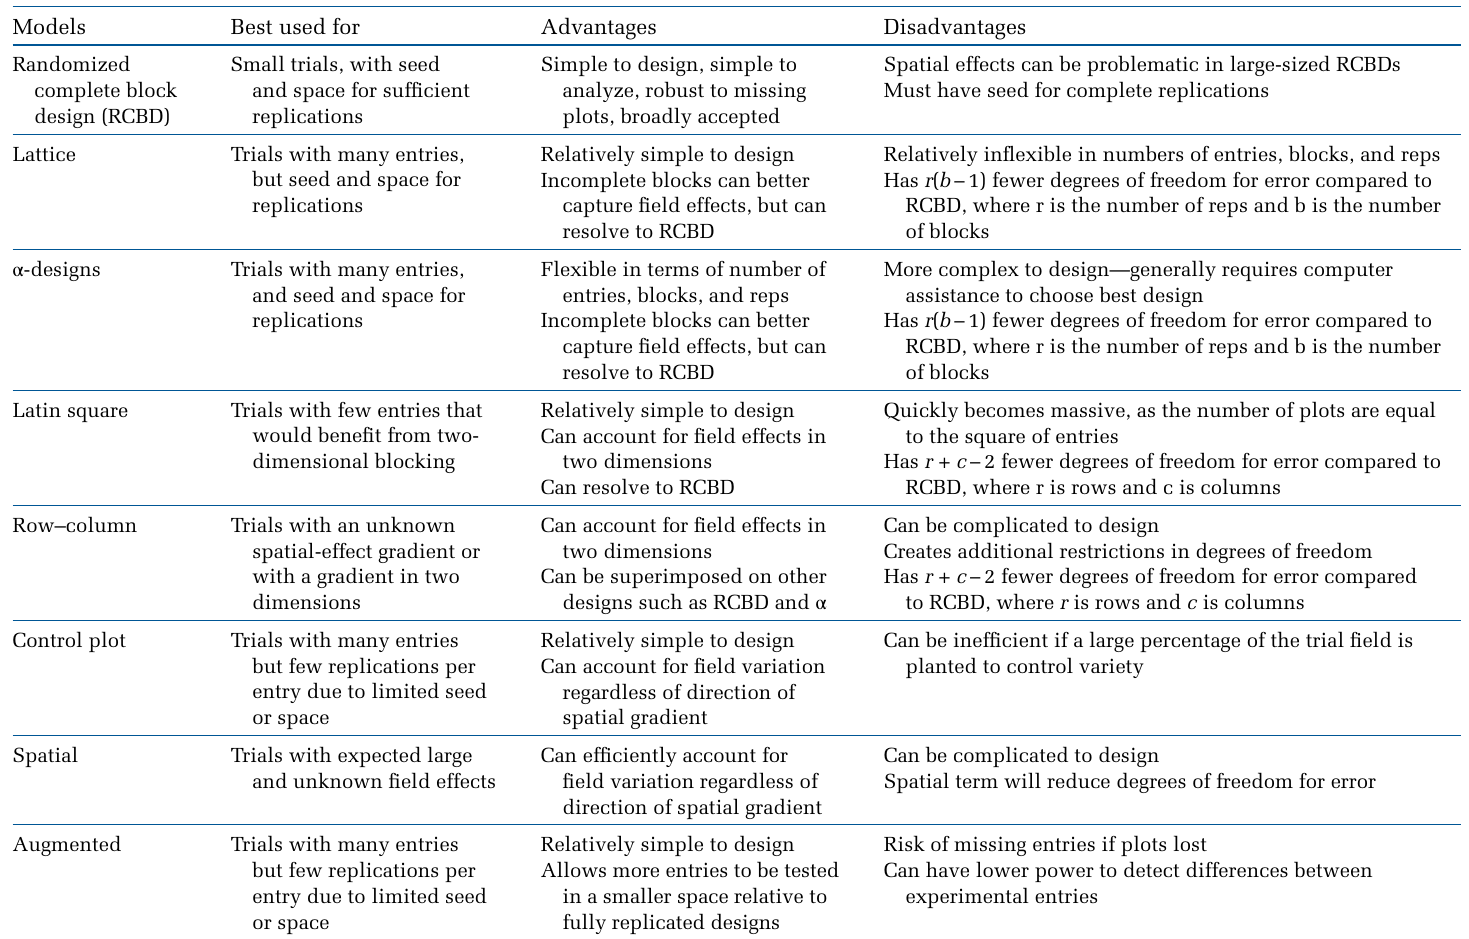
\includegraphics[width=0.7\linewidth]{./images/experimental-designs-comparison} \end{center}
\end{frame}

\hypertarget{bibliography}{%
\section{Bibliography}\label{bibliography}}

\begin{frame}{References}
\protect\hypertarget{references}{}
\end{frame}

\end{document}
